\documentclass{jarticle}

\usepackage{fancyhdr}
\usepackage[english]{babel}
\usepackage[dvipdfmx]{graphicx}
\usepackage{listings,jlisting}
\usepackage{here}

\setlength{\topmargin}{-10mm} % 15mm - 1in
\setlength{\headheight}{5mm}
\setlength{\headsep}{5mm}
\setlength{\oddsidemargin}{-7mm} % 18mm - 1in
\setlength{\evensidemargin}{-7mm} % 18mm - 1in
\setlength{\textheight}{247mm} % 297 - 25(top) - 25(bottom)
\setlength{\textwidth}{174mm} % 210 - 18*2
\setlength{\columnsep}{7mm}

\title{情報基礎1 最終レポート}
\author{坂本 嵩}
\date{\today}
\begin{document}
\maketitle

\section{はじめに}
\subsection{作成物} 自分の経歴や成果物をまとめた自己紹介ページ.	

\subsection{動機} 
将来研究者としての道を進むに当たって, 院進や就職の際, また学会発表などの後に "Shu Sakamoto", "坂本 嵩"で検索されることの増加が予想される. 研究者としての資質を見るため・単純に研究内容が気になったからなど理由は様々であろうが, 現在Google検索で表示されるFacebookページ/LinkedInページだけでは情報量に欠け, 正しく自身の像を伝えることができない. そのため, 自分の業績や経歴をより効果的に正しく伝えるページを作成し, これからの人生に少しでも役立てることが必要だと考えた.

\subsection{ボツになった候補とその理由}
\begin{enumerate}
	\item 
	ピンポンゲームなどの簡単なゲーム. 開発コストの高さと自身の将来への貢献度が釣り合わなかったため, ボツ.
	\item
	自分の趣味であるクラシック音楽 (特にチャイコフスキー) についてまとめ, 曲解説とともに視聴をできるようにしたページ. 将来への貢献度がほぼゼロに等しいため, ボツ.
\end{enumerate}

\section{設計}

Figure 1. がトップページとなる. トップページから各サブページに飛ぶと詳細の情報を閲覧できる. また, "Full-Screen Image Layer Viewer"\cite{ettrics}を使用して各セクションのタイトルにマウスを合わせると画像が変化するエフェクトを追加する. おしゃれなページにするために全画面に高画質な画像を表示し, 白文字もしくはグレー文字を使用する.

\begin{figure}[H]
  \begin{center}
    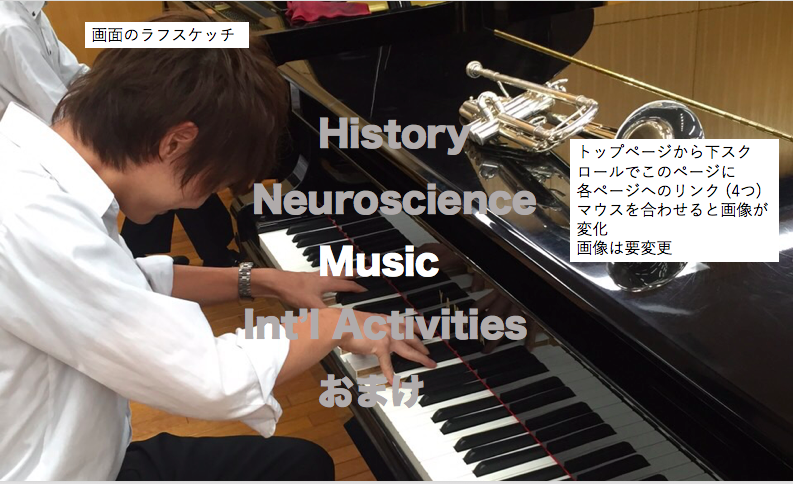
\includegraphics[clip,width=8cm]{./images/top_page_sketch.png}
    \caption{トップページのスケッチ.}
  \end{center}
\end{figure}


\section{実装}

\subsection{構造}
ディレクトリ構造は以下のようになっている
\begin{itemize}
	\item info1ディレクトリ...トップページ, 各サブページへのリンクを表示. リンクにマウスを合わせると背景画像が変化するアニメーションを追加.
			\begin{itemize}
				\item final.html
				\item final.js
				\item final.css
		\item educationディレクトリ... 'education'をクリックすると表示されるサブページ. 今までの学歴をまとめたもの.
			\begin{itemize}
				\item education.html
				\item subpage.css
			\end{itemize}
		\item neuroディレクトリ... 'neuroscience'をクリックすると表示されるサブページ. 脳科学研究の経歴や業績をまとめたもの
			\begin{itemize}
				\item neuro.html
				\item subpage.css
			\end{itemize}
		\item musicディレクトリ... 'music'をクリックすると表示されるサブページ. 音楽経験や所属団体をまとめたもの.
			\begin{itemize}
				\item music.html
				\item subpage.css
			\end{itemize}
		\item intlディレクトリ... 'int'l activities'をクリックすると表示されるサブページ. 海外経験や国際関係の活動についてまとめたもの.
			\begin{itemize}
				\item intl.html
				\item subpage.css
			\end{itemize}
		\item extraディレクトリ... 'おまけ'をクリックすると表示されるサブページ. おまけのゲームが二つ表示されたページ.
			\begin{itemize}
				\item extra.html
				\item extra.css
				\item extra.js
				\item aho.html
				\item aho.js
			\end{itemize}
		\item imagesディレクトリ... 画像ファイルを収納
		\item jquery-2.1.3.min.js
  \end{itemize}
\end{itemize}

\subsection{他から引用したもの}
\begin{enumerate}
	\item 
	トップページのアニメーションエフェクト, 及びテンプレート. final.htmlの15〜30行目, final.cssの22〜27行目以外, final.jsの全てはEttircs\cite{ettrics}よりテンプレートを使用した.
	\item 
	各サブページのぼかしエフェクト. subpage.cssの14-24, 39行目以外, extra.cssの14-24, 39, 68-73行目以外はsayuri\cite{sayuri}よりテンプレートを使用.
	\item
	jQuery-2.1.3を使用.
\end{enumerate}

\subsection{JavaScriptの説明}
指示通り一行ずつコメントを埋め込んだ.
\begin{enumerate}
	\item extra.js
		\begin{lstlisting}[basicstyle=\ttfamily\footnotesize,frame=single]
function prime(){ //素数判定をする前にinput値が数字のみで構成されているかをチェック
  // input値がintのみで構成されているかチェック
  var nStr = document.getElementById("primeOrNot").value; //input値を取ってくる
  var array = nStr.split(''); //inputを配列に分解
  for (var i=0, tf=0, l=array.length; i<l; i++){ //配列の要素を一つずつarray[i]としてチェック
    for (var j=0, c=0; j<10; j++){ //jを1から10までかぞえあげる
      if(array[i] != j){ // もし配列の要素がj(1-10)でなければ
        c += 1 //cに1を足す. array[i]が数字であれば1回だけこの行が無視される.
      }
    }
    if(c == 10){ //もしarray[i]のいずれかが1-10のどれでもなければ
      tf=1; //tfに1を代入する
      break //即座にfor文を終わらせ, 17行目に行く.
    }
  }
  //結果によって行動を変える
  if (tf == 1){ //もしtfが1なら, つまり1つでも1-10でない文字が入力されていたら
    alert("数値を入力してください"); //このメッセージを表示.
  } else { //もし数字のみが入力されていれば
    judgePrime(parseInt(nStr)); //strであるinput値をint型へと変換し,judgePrime()に受け渡す.
  }
}

function judgePrime(n){ //素数判定を行う関数
  //特別なケースに対処
  if(n <= 0){ //もし正の値が入力されていなければ
    alert("1以上の数値を入力してください"); //メッセージを表示
  } else if(n == 1){ //もしinput値が1ならば
    alert("素数ではありません"); //このメッセージを表示
  } else if(n == 2 || n == 3){ //もしinput値が2か3なら
    alert("素数"); //メッセージを表示
  } else{ //特殊なケースでなければ(4以上の値)
    for (var i=2, tf=0, limit=n**0.5; i<limit; i++ ){ //2からnの平方根まで数え上げ、
      if (n % i == 0){ //一つでもnを割り切れたら素数ではないので、
        alert("素数ではありません"); //メッセージを表示し、
        tf = 1; //tfに1を代入して
        break;//forループを即座に終了
      }
    }
    if (tf == 0){ //もしtfが0のままなら(forループを強制終了されることなくここまできたら)
      alert("素数"); //nは素数であるのでこのメッセージを表示
    }
  }
}

function aho(){ //アホ判定をする前にinput値が数字のみで構成されているかをチェック
  // input値がintのみで構成されているかチェック
  var nStr = document.getElementById("aho").value; //input値を取ってくる
  var array = nStr.split(''); //inputを配列に分解
  for (var i=0, tf=0, l=array.length; i<l; i++){ //配列の要素を一つずつarray[i]としてチェック
    for (var j=0, c=0; j<10; j++){ //jを1から10までかぞえあげる
      if(array[i] != j){ // もし配列の要素がj(1-10)でなければ
        c += 1 //cに1を足す. array[i]が数字であれば1回だけこの行が無視される.
      }
    }
    if(c == 10){ //もしarray[i]のいずれかが1-10のどれでもなければ
      tf=1; //tfに1を代入する
      break //即座にfor文を終わらせ, 17行目に行く.
    }
  }
  //結果によって行動を変える
  if (tf == 1){ //もしtfが1なら, つまり1つでも1-10でない文字が入力されていたら
    alert("数値を入力してください"); //このメッセージを表示.
  } else {
    judgeAho(parseInt(number));
  }
}

function judgeAho(n){ 
//お前がアホかどうかを判定してやるコード. 4の倍数か4が含まれていればアホなんやで.
  if (n%4 == 0){ //nが4の倍数なら
    beAho(); //アホやん!
  }else{ //nが4の倍数でなくでも
   var nStr =  String(n); //nをint型からstr型に変更し, 
   var array = nStr.split(''); //nを配列に分解
   for (var i=0, tf=0, l=array.length; i<l; i++){ //配列の要素を一つずつ見る.
    if(array[i]=="4"){ //もし一つでも4を含めば
      beAho(); //アホになる!
      tf=1; //tfを1とし, 
      break //即座にfor文を抜け出す
    }
   }
  }
  if (tf==0){ //もしtfが0のままなら
    notAho(); //ようやくアホじゃないことになる
  }
}

function beAho(){ //アホのアホによるアホのための関数
  var str = document.getElementById("message"); 
  //innerHTMLでメッセージを変更するのでidを取得
  str.innerHTML = "<span class='aho'>アホ!アホ!アホ!</span>"; 
  //innerHTMLでid="message"の部分を変更, <span></span>を用いて文字を装飾.
  window.open('./aho.html', '','width=500, height=400'); 
  //aho.html (アホ!と書かれたウィンドウ)をさらに追い打ちで開く. アホは徹底的に処罰する.
}

function notAho(){
  var str = document.getElementById("message"); //同じくinnerHTMLを使用
  str.innerHTML = "アホじゃない!"; //アホじゃない人には優しく
}



		\end{lstlisting}
	\item final.js
		\begin{lstlisting}[basicstyle=\ttfamily\footnotesize,frame=single]
var project = jQuery('.project'); //.project(css参照)をjQueryオブジェクトに指定
var pLink = project.find('.project__link'); //projectの中の.project__linkをpLinkに代入
var pBg = project.find('.project__bg-item'); //上記同様

var changeBg = function() { //背景画像を変える関数
  var thisProject = jQuery(this); //'mouseenter'されるpLinkをthisProjectに代入
  var thisProjectIndex = thisProject.parent().index();
  //thisProjectが.project_linkの親クラス==.project__listクラスで何番目か
  var thisProjectBg = pBg.eq(thisProjectIndex);
  // 上で取得したthisProjectIndex番目の.project__bg-item(html参照)を代入
  
  pBg.removeClass('project__bg-item--active');
  //一旦全てのリンクからactiveクラスを削除(前にactiveだったものを取り下げる)
  pLink.css('opacity', '0.4');
  //全てのリンクのスタイルも未選択状態にする(透明度を上げ, 目立ちやすくする)
  
  thisProject.css('opacity', '1'); 
  //そこからmouseenterされたリンクのスタイルを変える(透明度を下げ, 目立ちやすくする)
  thisProjectBg.addClass('project__bg-item--active');
  //activeクラスを追加, cssで指定されたtransformとopacityに.
};

var showFirst = function() { //ページがロード/リロードされたときの動き
  pLink.css('opacity', '0.4'); //全てのリンクのスタイルを一旦未選択状態に
  pLink.parent().first().children().css('opacity', '1');
  //pLinkの親クラス.project__listの一番最初の子クラス(.project__link)を選択状態に
  pBg.first().addClass('project__bg-item--active');//一番最初の.project__bg-itemをactiveに.
};

var init = function() {//実行する関数
  jQuery(document).on('ready', showFirst);//htmlの読み込みが終わったらshowFirstを実行
  pLink.on('mouseenter', changeBg);//pLinkのどれかがホバーされたらそのリンクにchangeBgを実行
};

init(); //実行
		\end{lstlisting}
  \item final.js
    \begin{lstlisting}[basicstyle=\ttfamily\footnotesize,frame=single]
var ahoCount = 0 //定義

function ahoClose(){ //ページを閉じようとしたアホを追撃する関数
  ahoCount += 1 //"ページを閉じる"をクリックした回数をカウントする
  var str = document.getElementById("aho"); //innerHTMLのidを取得
  for (i=0; i<ahoCount; i++){ //ページを閉じようとした回数分アホが増える
    str.innerHTML = str.innerHTML + "アホ!!!"; //innerHTMLでid="aho"の部分を変更.
  }
}

    \end{lstlisting}

\end{enumerate}

\section{評価}
自分の設計通りに関数は動き, 満足のいくページを作ることができた. 関数が思惑通り動かないこともあったが, それを直すのが非常に楽しかった. e.g.) extra.jsにあるinputが数字のみで構成されているかを判断する箇所. 当初は\begin{verbatim}type(input) == "string" \end{verbatim}や\begin{verbatim}input%1 == 0\end{verbatim}などで判断していたが, それだと上手くいかなかったためそのバグを直した.

自分の実績をある程度網羅するという目的は達成しているので, 現時点で改善するべき点はそれほどない. ただ, これから研究業績などができた際は論文や学会抄録のページに飛べるようリンクを作成すると便利だと思った. また, 余裕があれば英語ページも作成し, 英語⇔日本語切り替えボタンも作成したい. 

\begin{thebibliography}{2}
	\bibitem{ettrics} Ettrics. "Full-screen Image Layer Viewer". CodePen. https://codepen.io/ettrics/pen/zxexgQ (12月25日参照).
	\bibitem{sayuri}sayuri. "ぼかし+". CodePen. https://codepen.io/giraffeweb/pen/GmqNWr (12月25日参照). 
\end{thebibliography}


\section*{謝辞}
TAの糸田さん, SAの山田さんにはfinal.htmlにjQueryをうまく反映させる手助けを頂きました. ここに感謝の意を表します. 


\end{document}
